\newpage
\hypertarget{t2m close}{}
\subsection{Additional author handling}
\genHeader

\begin{itemize}

\item[$\blacktriangleright$] If your project's build succeeded, run \texttt{TGGMain} again and examine the forward direction's output, 
\texttt{tree.xmi\_FWD.xmi}, a little closer (Fig.~\ref{eclipse:generatedFwdTrsfm}).

\vspace{0.5cm}

\begin{figure}[htbp]
\begin{center}
  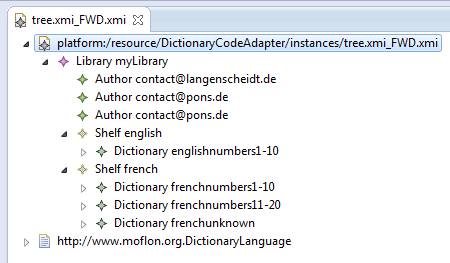
\includegraphics[width=0.7\textwidth]{eclipse_generatedForwardTransformation}
  \caption{\texttt{Dictionary} result of the forward transformation}
  \label{eclipse:generatedFwdTrsfm}
\end{center}
\end{figure}

\vspace{0.5cm}

\item[$\blacktriangleright$] Your output may or may not resemble ours. In fact, there's a 50/50 chance that some of the \texttt{author} nodes ever created!
Let's run the eMoflon integrator on \texttt{corr\_FWD.xmi} to find out why.\footnote{If you haven't already, read Part IV, Section 6 for details on how the
integrator can help you visualise and debug a transformation}

\vspace{0.5cm}

\item[$\blacktriangleright$] Proceed through the transformation until you reach the first match to an author node (Fig.~\ref{eclipse:fwdIntegrator}). Keep an
eye on the small window below -- it states that there are two possible rules that apply to the match!

\begin{figure}[htbp]
\begin{center}
  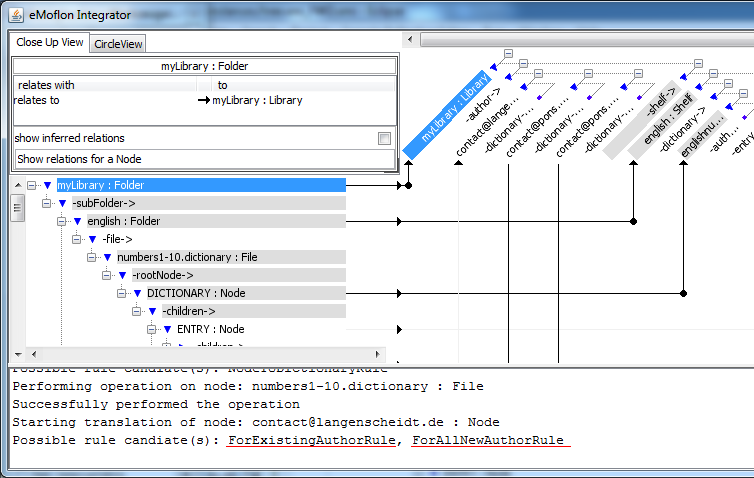
\includegraphics[width=0.8\textwidth]{eclipse_integratorAuthorChoice}
  \caption{The transformation is able to find two possible rules}
  \label{eclipse:fwdIntegrator}
\end{center}
\end{figure}

\clearpage

\item[$\blacktriangleright$] At run-time, the transformation is presented with a choice between two rules to apply to the matched \texttt{authorNode}. The
resulting choice is entirely random, meaning that your output is likely to be different each time you run \texttt{TGGMain}. For a deterministic transformation,
you therefore need to force a preferred decision. There are two ways to do this: (1) at run-time, where users will be able to decide for themselves what they would
prefer to use, or (2) at design-time, where you make the decision a part of the TGG.

\end{itemize}

\subsubsection{Option 1: Run-time decision}

The advantage with this option is that you give users the choice of what they prefer. Some users don't mind having multiple authors, while others might prefer a
minimalist design. They can easily change their preference possibly on a case-by-case basis, by implementing a TGG rule configurator.

\begin{itemize}

\item[$\blacktriangleright$] Navigate to ``DictionaryCodeAdapter/src/org.moflon.tie.'' Right-click this package and create a new java class named
\texttt{Author\-Config\-ur\-at\-or}, then complete the override as described in Fig.~\ref{eclipse:authorConfig}. Be careful not to make any mistakes --
Eclipse's auto-completion can help you here.

\begin{figure}[htbp]
\begin{center}
  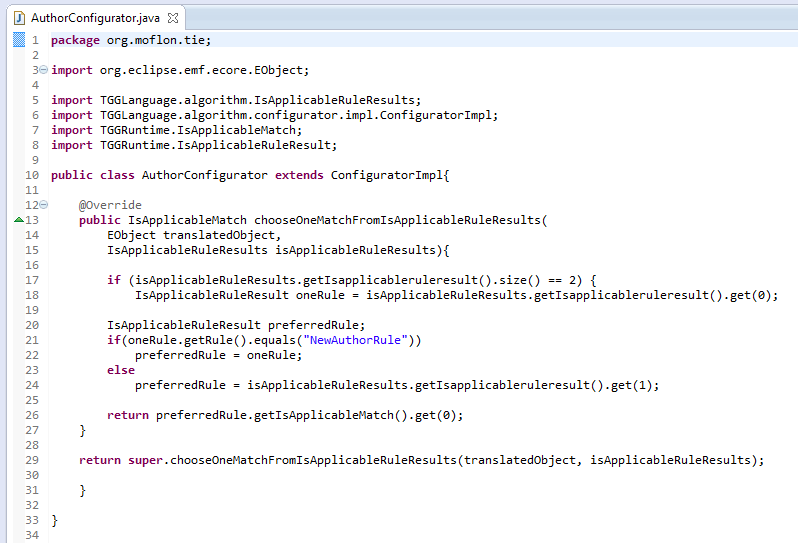
\includegraphics[width=\textwidth]{eclipse_authorConfiguratorClass}
  \caption{Setting a preference for \texttt{NewAuthorRule}}
  \label{eclipse:authorConfig}
\end{center}
\end{figure}

\clearpage

\item[$\blacktriangleright$] As you can see on Line 22, this simple configurator prefers to create a new author every time there is a choice. Users can
edit this value to ``ExistingAuthorRule'' to avoid redundant authors.

\item[$\blacktriangleright$] You still need to set the configurator to be used for the transformation. This decision will only arise in the forward
direction, so declare it once in \texttt{TGGMain/performForward} as depicted in Fig.~\ref{eclipse:editTGGMain} on Line 59.

\vspace{0.5cm}

\begin{figure}[htbp]
\begin{center}
  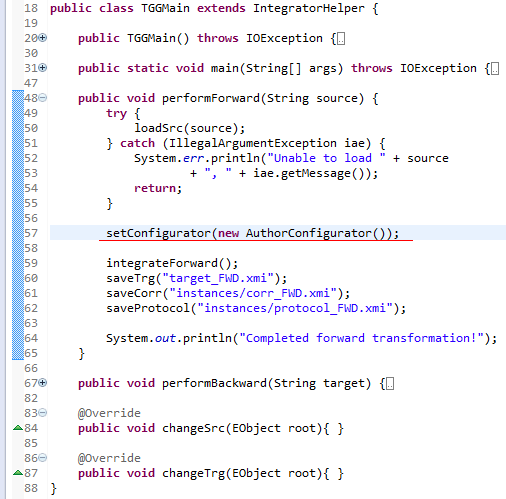
\includegraphics[width=\textwidth]{eclipse_authorConfiguratorTGGMain}
  \caption{Setting the configurator to control the run-time decision}
  \label{eclipse:editTGGMain}
\end{center}
\end{figure}

\end{itemize}

\subsubsection{Option 2: Design-time decision}

It is also possible to set a preference as part of the actual design of the transformation -- users will not be able to modify this. In our example, this
preference can be enforced using a NAC which checks to see if there is already an author with the same email in the library.

\begin{itemize}

\item[$\blacktriangleright$] Open and update either \texttt{NewAuthorRule} (visual) as shown in Fig.~\ref{ea:existingAuthorNAC} or edit the target domain in 
\texttt{ForAllNewAuthorRule.tgg} (textual) as depicted in Fig.~\ref{eclipse:existingAuthorNAC}.


\begin{figure}[htbp]
\begin{center}
  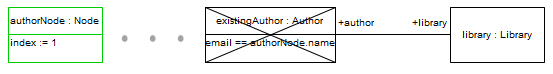
\includegraphics[width=\textwidth]{ea_NewAuthorRuleNAC}
  \caption{Refine \texttt{AuthorRule} by adding a NAC in \texttt{NewAuthorRule} \update}
  \label{ea:existingAuthorNAC}
\end{center}
\end{figure}

\begin{figure}[htbp]
\begin{center}
  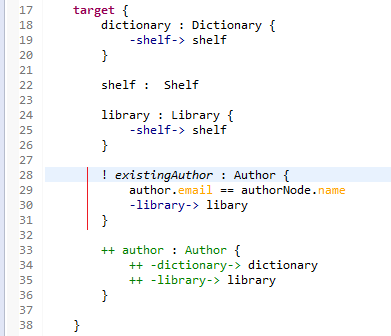
\includegraphics[width=0.7\textwidth]{eclipse_ForAllNewAuthorNAC}
  \caption{Add a NAC to \texttt{ForAllNewAuthorRule}}
  \label{eclipse:existingAuthorNAC}
\end{center}
\end{figure}

\item[$\blacktriangleright$] Save and rebuild the TGG. Run the transformation a few times, using the integrator to confirm that your preference (no redudant
authors are created) is enforced each time. 

\end{itemize}

Let's examine the results! First, You'll notice that, as you scroll through each \texttt{Node}, the \texttt{title} and \texttt{author} nodes have the correct
\texttt{index} values of 0 and 1, but the remaining \texttt{entry} indices are also set to 0. We were only concerned with binding the title and author nodes in
the forward direction, as we could assume that any other node with any other index value (2 and greater) was an \texttt{entryNode}. In the backwards direction
however, this distinction is lost, which means we must introduce a custom attribute constraint.
